\documentclass{beamer}
\usepackage[utf8]{inputenc}
\usepackage[T1]{fontenc}
\usepackage[english]{babel}
\usepackage{graphicx}
\usepackage{times}
\usepackage{algorithm}
\usepackage{algpseudocode}
\usepackage{amsmath}
\usepackage{amssymb}
\usepackage{tikz}
\usetikzlibrary{calendar} 
\usetikzlibrary{calc,through,backgrounds,positioning,fit}
\usetikzlibrary{shapes,arrows,shadows,calendar}
\title{Beamer}
\author[A.Iksiński]{A.Iksiński}
\institute{Wydział EAIiIB\\Katedra Informatyki Stosowanej}
\date[PL’06]{2015}
\subject{Beamer}
\usetheme{Darmstadt}

 

\begin{document}
\begin{frame}
\titlepage
\end{frame}
 
%--------------------------------------------------
 
\begin{frame}[fragile, t]    % fragile!!!, bo używamy verb

\frametitle{Algorytm}
\begin{algorithmic}
\State $\triangleright$ \verb!ASSIGN! 
\end{algorithmic}
 
\end{frame}
 
%--------------------------------------------------
\begin{frame}[fragile, t]    % fragile!!!, bo używamy verb

\frametitle{Algorytm}
\begin{algorithmic}
\State $\triangleright$ \verb!ASSIGN! 
\State $\triangleright$ \verb!init(s) = s0!

\end{algorithmic}
 
\end{frame}
 
%--------------------------------------------------
\begin{frame}[fragile, t]    % fragile!!!, bo używamy verb

\frametitle{Algorytm}
\begin{algorithmic}
\State $\triangleright$ \verb!ASSIGN! 
\State $\triangleright$ \verb!init(s) = s0!

\end{algorithmic}
 
\end{frame}
 
%--------------------------------------------------
\begin{frame}[fragile, t]    % fragile!!!, bo używamy verb

\frametitle{Algorytm}
\begin{algorithmic}
\State $\triangleright$ \verb!ASSIGN!
\State $\triangleright$ \verb!init(s) = s0!
\State $\triangleright$ \verb!next(s) := case!

\end{algorithmic}
 
\end{frame}
 
%--------------------------------------------------
\begin{frame}[fragile, t]    % fragile!!!, bo używamy verb

\frametitle{Algorytm}
\begin{algorithmic}
\State $\triangleright$ \verb!ASSIGN!
\State $\triangleright$ \verb!init(s) = s0!
\State $\triangleright$ \verb!next(s) := case!
\ForAll{$si \in s$}

\end{algorithmic}
 
\end{frame}
 
%--------------------------------------------------
\begin{frame}[fragile, t]    % fragile!!!, bo używamy verb

\frametitle{Algorytm}
\begin{algorithmic}
\State $\triangleright$ \verb!ASSIGN!
\State $\triangleright$ \verb!init(s) = s0!
\State $\triangleright$ \verb!next(s) := case!
\ForAll{$si \in s$}
   \ForAll{$tk \in T$} 
   		
\end{algorithmic}
 
\end{frame}
 
%--------------------------------------------------
\begin{frame}[fragile, t]    % fragile!!!, bo używamy verb

\frametitle{Algorytm}
\begin{algorithmic}
\State $\triangleright$ \verb!ASSIGN!
\State $\triangleright$ \verb!init(s) = s0!
\State $\triangleright$ \verb!next(s) := case!
\ForAll{$si \in s$}
   \ForAll{$tk \in T$} 
   		\State $V_{ik} \gets \emptyset$ 
   		
\end{algorithmic}
 
\end{frame}
 
%--------------------------------------------------
\begin{frame}[fragile, t]    % fragile!!!, bo używamy verb

\frametitle{Algorytm}
\begin{algorithmic}
\State $\triangleright$ \verb!ASSIGN!
\State $\triangleright$ \verb!init(s) = s0!
\State $\triangleright$ \verb!next(s) := case!
\ForAll{$si \in s$}
   \ForAll{$tk \in T$} 
   		\State $V_{ik} \gets \emptyset$ 
   		\ForAll{$sj \in s$} 
   			
\end{algorithmic}
 
\end{frame}
 
%--------------------------------------------------
\begin{frame}[fragile, t]    % fragile!!!, bo używamy verb

\frametitle{Algorytm}
\begin{algorithmic}
\State $\triangleright$ \verb!ASSIGN!
\State $\triangleright$ \verb!init(s) = s0!
\State $\triangleright$ \verb!next(s) := case!
\ForAll{$si \in s$}
   \ForAll{$tk \in T$} 
   		\State $V_{ik} \gets \emptyset$ 
   		\ForAll{$sj \in s$} 
   			\If {$(M_{i},S_{i})\overset{tk}{\longrightarrow}(M_{j},S_{j})$}
   				
\end{algorithmic}
 
\end{frame}
 
%--------------------------------------------------
\begin{frame}[fragile, t]    % fragile!!!, bo używamy verb

\frametitle{Algorytm}
\begin{algorithmic}
\State $\triangleright$ \verb!ASSIGN!
\State $\triangleright$ \verb!init(s) = s0!
\State $\triangleright$ \verb!next(s) := case!
\ForAll{$si \in s$}
   \ForAll{$tk \in T$} 
   		\State $V_{ik} \gets \emptyset$ 
   		\ForAll{$sj \in s$} 
   			\If {$(M_{i},S_{i})\overset{tk}{\longrightarrow}(M_{j},S_{j})$}
   				\State $V_{ik} \gets V_{ik} \cup\{sj\}$
   			
\end{algorithmic}
 
\end{frame}
 
%--------------------------------------------------
\begin{frame}[fragile, t]    % fragile!!!, bo używamy verb

\frametitle{Algorytm}
\begin{algorithmic}
\State $\triangleright$ \verb!ASSIGN!
\State $\triangleright$ \verb!init(s) = s0!
\State $\triangleright$ \verb!next(s) := case!
\ForAll{$si \in s$}
   \ForAll{$tk \in T$} 
   		\State $V_{ik} \gets \emptyset$ 
   		\ForAll{$sj \in s$} 
   			\If {$(M_{i},S_{i})\overset{tk}{\longrightarrow}(M_{j},S_{j})$}
   				\State $V_{ik} \gets V_{ik} \cup\{sj\}$
   			\EndIf
   		
\end{algorithmic}
 
\end{frame}
 
%--------------------------------------------------
\begin{frame}[fragile, t]    % fragile!!!, bo używamy verb

\frametitle{Algorytm}
\begin{algorithmic}
\State $\triangleright$ \verb!ASSIGN!
\State $\triangleright$ \verb!init(s) = s0!
\State $\triangleright$ \verb!next(s) := case!
\ForAll{$si \in s$}
   \ForAll{$tk \in T$} 
   		\State $V_{ik} \gets \emptyset$ 
   		\ForAll{$sj \in s$} 
   			\If {$(M_{i},S_{i})\overset{tk}{\longrightarrow}(M_{j},S_{j})$}
   				\State $V_{ik} \gets V_{ik} \cup\{sj\}$
   			\EndIf
   		\EndFor
   		
\end{algorithmic}
 
\end{frame}
 
%--------------------------------------------------
\begin{frame}[fragile, t]    % fragile!!!, bo używamy verb

\frametitle{Algorytm}
\begin{algorithmic}
\State $\triangleright$ \verb!ASSIGN!
\State $\triangleright$ \verb!init(s) = s0!
\State $\triangleright$ \verb!next(s) := case!
\ForAll{$si \in s$}
   \ForAll{$tk \in T$} 
   		\State $V_{ik} \gets \emptyset$ 
   		\ForAll{$sj \in s$} 
   			\If {$(M_{i},S_{i})\overset{tk}{\longrightarrow}(M_{j},S_{j})$}
   				\State $V_{ik} \gets V_{ik} \cup\{sj\}$
   			\EndIf
   		\EndFor
   		\State $\triangleright$ \verb!s = si & action = tk:! $\{V_{ik}contents\};$
   
\end{algorithmic}
 
\end{frame}
 
%--------------------------------------------------
\begin{frame}[fragile, t]    % fragile!!!, bo używamy verb

\frametitle{Algorytm}
\begin{algorithmic}
\State $\triangleright$ \verb!ASSIGN!
\State $\triangleright$ \verb!init(s) = s0!
\State $\triangleright$ \verb!next(s) := case!
\ForAll{$si \in s$}
   \ForAll{$tk \in T$} 
   		\State $V_{ik} \gets \emptyset$ 
   		\ForAll{$sj \in s$} 
   			\If {$(M_{i},S_{i})\overset{tk}{\longrightarrow}(M_{j},S_{j})$}
   				\State $V_{ik} \gets V_{ik} \cup\{sj\}$
   			\EndIf
   		\EndFor
   		\State $\triangleright$ \verb!s = si & action = tk:! $\{V_{ik}contents\};$
   	\EndFor

\end{algorithmic}
 
\end{frame}
 
%--------------------------------------------------
\begin{frame}[fragile, t]    % fragile!!!, bo używamy verb

\frametitle{Algorytm}
\begin{algorithmic}
\State $\triangleright$ \verb!ASSIGN!
\State $\triangleright$ \verb!init(s) = s0!
\State $\triangleright$ \verb!next(s) := case!
\ForAll{$si \in s$}
   \ForAll{$tk \in T$} 
   		\State $V_{ik} \gets \emptyset$ 
   		\ForAll{$sj \in s$} 
   			\If {$(M_{i},S_{i})\overset{tk}{\longrightarrow}(M_{j},S_{j})$}
   				\State $V_{ik} \gets V_{ik} \cup\{sj\}$
   			\EndIf
   		\EndFor
   		\State $\triangleright$ \verb!s = si & action = tk:! $\{V_{ik}contents\};$
   \EndFor
\EndFor
\State $\triangleright$ \verb!esac;!
\end{algorithmic}
 
\end{frame}
 
 
%--------------------------------------------------
 
\begin{frame}
\frametitle{Zadanie 5.1}
 
 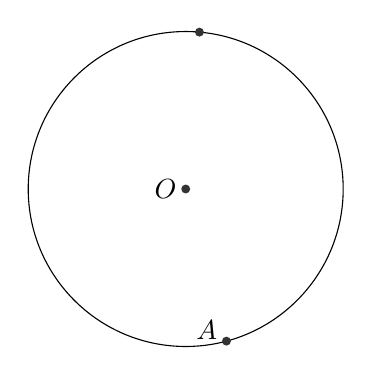
\begin{tikzpicture}[scale=1,inner sep=0.4mm]

\coordinate (O) at (0,0);
\coordinate (A) at (-75:2cm);
\coordinate (B) at (85:2cm);
\draw (0,0) circle (2cm);
\node at (O) [circle,fill=black!80!white] {};
\node at (A) [circle,fill=black!80!white] {};
\node at (B) [circle,fill=black!80!white] {};

-
% ...
\node at (O) [left=2pt] {$O$};
\node at (A) [left=2pt, yshift=4pt] {$A$};

% ...
\end{tikzpicture}
\end{frame}

%--------------------------------------------------
 
\begin{frame}
\frametitle{Zadanie 5.1}
 
 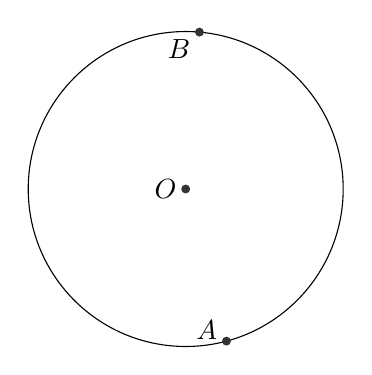
\begin{tikzpicture}[scale=1,inner sep=0.4mm]

\coordinate (O) at (0,0);
\coordinate (A) at (-75:2cm);
\coordinate (B) at (85:2cm);
\draw (0,0) circle (2cm);
\node at (O) [circle,fill=black!80!white] {};
\node at (A) [circle,fill=black!80!white] {};
\node at (B) [circle,fill=black!80!white] {};

-
% ...
\node at (O) [left=2pt] {$O$};
\node at (A) [left=2pt, yshift=4pt] {$A$};
\node at (B) [left=2pt, yshift=-6pt] {$B$};

% ...
\end{tikzpicture}
\end{frame}
%--------------------------------------------------
 
\begin{frame}
\frametitle{Zadanie 5.1}
 
 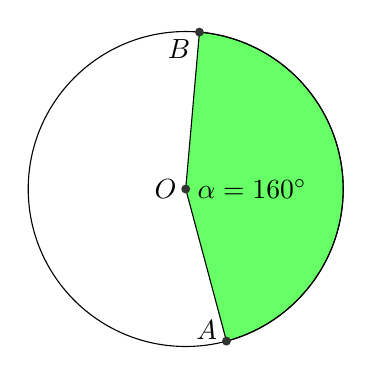
\begin{tikzpicture}[scale=1,inner sep=0.4mm]
\fill[green!60!white, draw=black](0,0) -- (-75:2) arc (-75:85:2) --cycle;
\coordinate (O) at (0,0);
\coordinate (A) at (-75:2cm);
\coordinate (B) at (85:2cm);
\draw (0,0) circle (2cm);
\node at (O) [circle,fill=black!80!white] {};
\node at (A) [circle,fill=black!80!white] {};
\node at (B) [circle,fill=black!80!white] {};

-
% ...
\node at (O) [left=2pt] {$O$};
\node at (A) [left=2pt, yshift=4pt] {$A$};
\node at (B) [left=2pt, yshift=-6pt] {$B$};
\node at (O) [right=3pt] {$\alpha = 160^{\circ}$};
% ...
\end{tikzpicture}
\end{frame}
 
%--------------------------------------------------
\begin{frame}
\frametitle{Kalendarz}

\begin{columns}
\column{0.45\textwidth}

\begin{block}{Styczeń 2015}
   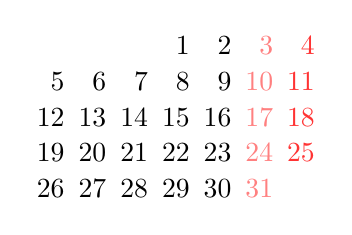
\begin{tikzpicture}
    \calendar[dates=2015-01-01 to 2015-01-31,week list]
    if (Sunday)            [red!80]
    if (Saturday)          [red!50];
    \end{tikzpicture}
    
\end{block}

\column{0.5\textwidth}
\only<2>{
  \begin{block}{Luty 2015}
  
     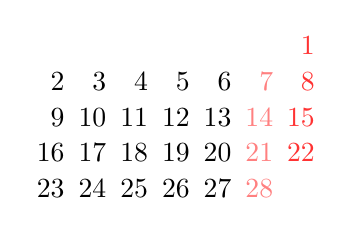
\begin{tikzpicture}
     \calendar[dates=2015-02-01 to 2015-02-28,week list]
      if (Sunday)            [red!80]
      if (Saturday)          [red!50];
      \end{tikzpicture}
  \end{block}
  }
  \end{columns}
\end{frame}

\begin{frame}
\frametitle{Kalendarz}
 
\begin{columns}
\column{0.45\textwidth}
\begin{block}{Styczeń 2015}
   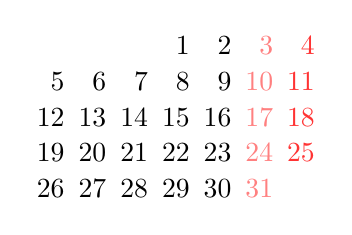
\begin{tikzpicture}
    \calendar[dates=2015-01-01 to 2015-01-31,week list]
    if (Sunday)            [red!80]
    if (Saturday)          [red!50];
    \end{tikzpicture}

\end{block}
\column{0.5\textwidth}

  \begin{block}{Marzec 2015}
     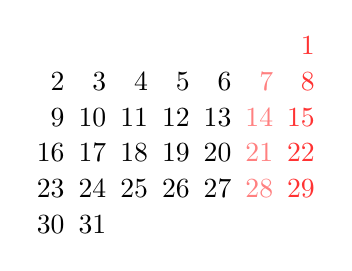
\begin{tikzpicture}
      \calendar[dates=2015-03-01 to 2015-03-31,week list]
      if (Sunday)            [red!80]
      if (Saturday)          [red!50];
      \end{tikzpicture}
  \end{block}

  
  \end{columns}
\end{frame}

\begin{frame}
\frametitle{Kalendarz}
 
\begin{columns}
\column{0.45\textwidth}
\begin{block}{Styczeń 2015}
   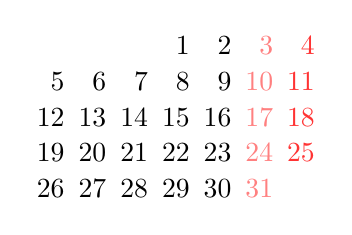
\begin{tikzpicture}
    \calendar[dates=2015-01-01 to 2015-01-31,week list]
    if (Sunday)            [red!80]
    if (Saturday)          [red!50];
    \end{tikzpicture}

\end{block}
\column{0.5\textwidth}

  \begin{block}{Kwiecień 2015}
     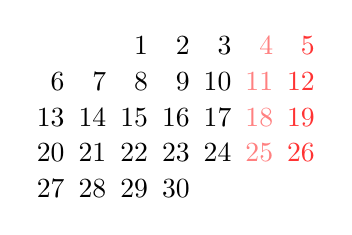
\begin{tikzpicture}
       \calendar[dates=2015-04-01 to 2015-04-30,week list]
      if (Sunday)            [red!80]
      if (Saturday)          [red!50];
      \end{tikzpicture}
  \end{block}

  
  \end{columns}
\end{frame}
  
  

 
\end{document}
 
 
 